\documentclass[a4paper, 12pt]{article}
\usepackage{amsmath}
\usepackage{csvsimple}
\usepackage{graphicx}
\usepackage{pdfpages}
\usepackage{etoolbox}
\usepackage{caption}
\usepackage{listings}
\usepackage[margin=1.0in]{geometry}
\usepackage{color}
\DeclareFixedFont{\ttb}{T1}{txtt}{bx}{n}{12} % for bold
\DeclareFixedFont{\ttm}{T1}{txtt}{m}{n}{12}  % for normal


\definecolor{mygreen}{rgb}{0,0.6,0}
\definecolor{mygray}{rgb}{0.5,0.5,0.5}
\definecolor{mymauve}{rgb}{0.58,0,0.82}

\lstset{ %
  backgroundcolor=\color{white},   % choose the background color
  basicstyle=\ttm,        % size of fonts used for the code
  breaklines=true,                 % automatic line breaking only at whitespace
  captionpos=b,                    % sets the caption-position to bottom
  commentstyle=\ttm\color{gray},    % comment style
  escapeinside={\%*}{*)},          % if you want to add LaTeX within your code
  keywordstyle=\ttb\color{blue},       % keyword style
  stringstyle=\ttm\color{mygreen},     % string literal style
}
\patchcmd{\thebibliography}{\section*{\refname}}{}{}{}
\begin{document}
\title{ME-429-101\\Controls and Instrumentation Lab\\Lab 10: Piezoelectric Accelerometer}
\date{11/12/18}
\author{Josh Fowler, Tyler Kendrick, Kanan Aljeneede}
\maketitle
\begin{figure}[h!tb]
\centering\noindent\makebox[\linewidth]{\rule{16cm}{0.4pt}}\\
\centering\noindent\makebox[\linewidth]{\rule{16cm}{0.4pt}}
\end{figure}
\section*{Author Contributions}
Josh Fowler (33 \%): Attended Lab, Performed Analysis, Recorded Data, Constructed Appendix\\
Tyler Kendrick (33 \%): Attended Lab, Measured Data, Set up Experiment, Wrote Body\\
Kanan Aljeneede (33 \%): Attended Lab, Constructed Circuits, Wrote Body\\
\section*{Statement of Quality}
This Report is an original work of the above mentioned authors.\\\\\\
\noindent\begin{tabular}{ll}\makebox[2.5in]{\hrulefill} &\makebox[2.5in]{\hrulefill}\\
Author & Date\\[8ex]\makebox[2.5in]{\hrulefill} &\makebox[2.5in]{\hrulefill}\\
Author & Date\\[8ex]\makebox[2.5in]{\hrulefill} &\makebox[2.5in]{\hrulefill}\\
Author & Date\\[8ex]\end{tabular}
\thispagestyle{empty}
\newpage
\tableofcontents
\thispagestyle{empty}
\newpage
\pagenumbering{arabic}
\section{: Introduction}
The purpose of the lab was to experimentally determine the flexural stiffness, (EI), of a sample of aluminum, and from our calculated moment of inertia, (I), the Young's Modulus, (E), as well as determine if our accelerometer was calibrated correctly. The modulus of elasticity is an important engineering characteristic used in many structural and modal problems, and thus calculating it for a sample that will be used in testing is quite useful.
\section{: Theory and Methods}
The dimensions of the sample of aluminum was measured to be 10in x 1/8 in x 1in, and the mass 66.12 g. The accelerometer's mass was determined to be 10.6g. A linear density was calculated by multiplying the reciprocal of the cross-sectional area by the mass of the aluminum beam and an equivalent mass was calculated. By attaching the accelerometer to the end of the beam, the voltage can be used to determine the acceleration, in G's, using the manufacturer's prescribed calibration. In order to determine the flexural stiffness of the aluminum sample we had to first set up the Data Acquisition System (DAQ). It is important to note that the sampling rate of the DAQ must be at least twice the frequency of the beam. After a few calibration runs to determine that there was no aliasing occurring, the sampling rate of the DAQ was set to 100 Hz, which was determined to be adequate for our experiment.\\\\
\section{: Results}
The results of our analysis were obtained using the data collected in the lab and compared to a solution using the finite element method with 5 elements, leading to a total of 10 natural frequencies and mode shapes determined. The data collected was Fast Fourier Transformed and the peak was used to find the corresponding frequency, 168.47 rad/s, (26.75 Hz), for the Damped Natural Frequency. Using exponential regression, the Natural Frequency was determined from the damped natural frequency as 180.4 rad/s or 28.7 Hz. Using the Finite Element method, it was determined that based on the tabulated value for the Young's Modulus of 6061 Aluminum, the natural frequency for our beam including the accelerometer should have been near 243.4 rad/s, (38.7 Hz). It was also determined that the flexural stiffness was $5.6 \pm 0.8 \frac{N}{m^2}$, using our calculated value for I, the Young's Modulus was determined to be, $64.8 \pm 5.9 GPa$, which was 27 GPa higher than the tabulated value. The modes for the first 4 natural frequencies were also calculated using the Finite Element Method, by finding the eigenvectors, and are shown below in Figures 5-10, using the sign changes for each node.
\section{: Conclusions and Recommendations}
The peak acceleration that the bar achieved was 5.2 G's, which seems reasonable on the surface. From our regression analysis the Predictive Model developed is quite good when using the calculated displacements. From the plot of our Experimental data to our Predictive Model, our calculated displacements are off by a factor of about 10 from the initial values recorded in the lab. The density that was calculated was also lower than what was expected for 6061 Aluminum, however was still in an acceptable range. The Finite Element Solution was about 10 Hz higher than our calculated values. We can conclude that if a higher number of elements was used, we could improve the solution, using 10 elements the solution converged to 28.7 Hz as the natural frequency of the beam, using our calculated values for the flexural stiffness.\\\\
In order to improve our results, we could attempt to come up with a solution to the wire from the accelerometer hitting the beam as it deflects. We attempted to tape the wire out of the way however, we were still getting noise from it. We could also use three clamps, one to hold it in place, and the other two on the side of the sample to keep it from moving. Even though the clamp was tightened as far as possible, as the beam vibrated the clamp moved slightly, allow the sample to move slightly to one side. Another improvement would that would have been possible if time permitted would be to use a filter on the output to dampen out the noise we were receiving. A different accelerometer that was calculated correctly would have improved data as well.

\appendix
\section*{Appendix}
\section{: Collected Data}
\begin{center}
\captionof{table}{Time vs Amplitude Run 1\protect\footnotemark}
\footnotetext{Due to the size of this data set, this table has been abbreviated}
\begin{tabular}{|l|l|}\hline
0.0&-0.00303712\\ \hline
0.001&-0.0027081\\ \hline
0.002&-0.00303712\\ \hline
0.003&-0.0027081\\ \hline
0.004&-0.00303712\\ \hline
0.005&-0.00336614\\ \hline
.&.\\
.&.\\
.&.\\
3.993&-0.00139203\\ \hline
3.994&-0.00139203\\ \hline
3.995&-0.00139203\\ \hline
3.996&-0.00139203\\ \hline
3.997&-0.00172105\\ \hline
3.998&-0.00139203\\ \hline
	\end{tabular}
\end{center}
\newpage
\begin{center}
\captionof{table}{Time vs Amplitude FFT Run 1\protect\footnotemark}
\footnotetext{Due to the size of this data set, this table has been abbreviated}
\begin{tabular}{|l|l|}\hline
0.0&-0.00303712\\ \hline
0.001&-0.0027081\\ \hline
0.002&-0.00303712\\ \hline
0.003&-0.0027081\\ \hline
0.004&-0.00336614\\ \hline
0.005&-0.00303712\\ \hline
.&.\\
.&.\\
.&.\\
3.993&-0.00172105\\ \hline
3.994&-0.00172105\\ \hline
3.995&-0.00139203\\ \hline
3.996&-0.00172105\\ \hline
3.997&-0.00139203\\ \hline
3.998&-0.00139203\\ \hline
	\end{tabular}
\end{center}
\begin{center}
\captionof{table}{Time vs Amplitude Run 2\protect\footnotemark}
\footnotetext{Due to the size of this data set, this table has been abbreviated}
\begin{tabular}{|l|l|}\hline
0.0&-0.00402418\\ \hline
0.001&-0.00369516\\ \hline
0.002&-0.00369516\\ \hline
0.003&-0.00369516\\ \hline
0.004&-0.00402418\\ \hline
0.005&-0.00369516\\ \hline
.&.\\
.&.\\
.&.\\
3.993&-0.00172105\\ \hline
3.994&-0.00237908\\ \hline
3.995&-0.00139203\\ \hline
3.996&-0.00237908\\ \hline
3.997&-0.00237908\\ \hline
3.998&-0.0027081\\ \hline
	\end{tabular}
\end{center}
\newpage
\begin{center}
\captionof{table}{Time vs Amplitude FFT Run 2\protect\footnotemark}
\footnotetext{Due to the size of this data set, this table has been abbreviated}
\begin{tabular}{|l|l|}\hline
0.0&-0.00369516\\ \hline
0.001&-0.00336614\\ \hline
0.002&-0.00303712\\ \hline
0.003&-0.00303712\\ \hline
0.004&-0.00303712\\ \hline
0.005&-0.0027081\\ \hline
.&.\\
.&.\\
.&.\\
3.993&-0.00402418\\ \hline
3.994&-0.00369516\\ \hline
3.995&-0.00303712\\ \hline
3.996&-0.00303712\\ \hline
3.997&-0.00369516\\ \hline
3.998&-0.00303712\\ \hline
	\end{tabular}
\end{center}
\begin{center}
\captionof{table}{Time vs Amplitude Run 3\protect\footnotemark}
\footnotetext{Due to the size of this data set, this table has been abbreviated}
\begin{tabular}{|l|l|}\hline
0.0&0.0036591\\ \hline
0.25&0.00248926\\ \hline
0.5&5.37e-05\\ \hline
0.75&6.04e-05\\ \hline
1.0&5.42e-05\\ \hline
1.25&8.98e-05\\ \hline
.&.\\
.&.\\
.&.\\
38.5&0.00011908\\ \hline
38.75&0.000160297\\ \hline
39.0&0.000129396\\ \hline
39.25&0.000106692\\ \hline
39.5&0.000217568\\ \hline
39.75&0.00031329\\ \hline
	\end{tabular}
\end{center}
\newpage
\begin{center}
\captionof{table}{Time vs Amplitude FFT Run 3\protect\footnotemark}
\footnotetext{Due to the size of this data set, this table has been abbreviated}
\begin{tabular}{|l|l|}\hline
0.0&0.00380653\\ \hline
0.25&0.00277308\\ \hline
0.5&0.00014633\\ \hline
0.75&9.78e-05\\ \hline
1.0&5.02e-05\\ \hline
1.25&7.68e-05\\ \hline
.&.\\
.&.\\
.&.\\
38.5&0.00062031\\ \hline
38.75&0.000626422\\ \hline
39.0&0.000489179\\ \hline
39.25&0.000491637\\ \hline
39.5&0.000667836\\ \hline
39.75&0.000771899\\ \hline
	\end{tabular}
\end{center}
\begin{center}
\captionof{table}{Time vs Amplitude Run 4\protect\footnotemark}
\footnotetext{Due to the size of this data set, this table has been abbreviated}
\begin{tabular}{|l|l|}\hline
0.0&0.00412772\\ \hline
0.25&0.00301049\\ \hline
0.5&0.000124944\\ \hline
0.75&8.87e-05\\ \hline
1.0&8.95e-05\\ \hline
1.25&0.00010309\\ \hline
.&.\\
.&.\\
.&.\\
38.25&0.000408575\\ \hline
38.5&0.000302626\\ \hline
38.75&0.000199188\\ \hline
39.0&0.000162791\\ \hline
39.25&0.000214143\\ \hline
39.5&0.000280749\\ \hline
	\end{tabular}
\end{center}
\newpage
\begin{center}
\captionof{table}{Time vs Amplitude FFT Run 4\protect\footnotemark}
\footnotetext{Due to the size of this data set, this table has been abbreviated}
\begin{tabular}{|l|l|}\hline
0.0&0.00391427\\ \hline
0.25&0.00284933\\ \hline
0.5&0.000129389\\ \hline
0.75&8.74e-05\\ \hline
1.0&5.12e-05\\ \hline
1.25&6.36e-05\\ \hline
.&.\\
.&.\\
.&.\\
38.25&0.00033297\\ \hline
38.5&0.000282793\\ \hline
38.75&0.000271477\\ \hline
39.0&0.000230445\\ \hline
39.25&0.00025218\\ \hline
39.5&0.000319506\\ \hline
	\end{tabular}
\end{center}
\section{: Equations}
\subsection{: Shape Functions}
\begin{equation}
N_1 = \frac{1}{L^3} \left( 2x^3 - 3x^2 L + L^3 \right)
\end{equation}
\begin{equation}
N_2 = \frac{1}{L^3} \left( x^3 - 2x^2 L^2 + xL^3 \right)
\end{equation}
\begin{equation}
N_3 = \frac{1}{L^3} \left(-2 x^3 +3x^2 L^2 \right)
\end{equation}
\begin{equation}
N_4 = \frac{1}{L^3} \left( x^3 L - x^2 L^2 \right)
\end{equation}
\begin{equation}
\left[ B \right] = -y \left[
\begin{matrix}
\frac{\partial^2 N_1}{\partial x^2} & \frac{\partial^2 N_2}{\partial x^2} & \frac{\partial^2 N_3}{\partial x^2} & \frac{\partial^2 N_4}{\partial x^2}
\end{matrix}
\right]
\end{equation}
\begin{equation}
\left[ D \right] = \left[ \Omega \left( x \right) \right]
\end{equation}
\begin{center}
where $ \left[ \Omega \left( x \right) \right] $ is some chosen weighted cubic displacement function.
\end{center}
\subsection{: Beam Element Continuous Mass Matrix}
\begin{equation}
\left[ m^{\left( e \right)} \right] = \int_0^L \iint_A \rho \left\{
\begin{matrix}
N_1 \\ N_2 \\ N_3 \\ N_4
\end{matrix} \right\}
\left[
\begin{matrix}
N_1 & N_2 & N_3 & N_4
\end{matrix}
\right] \, dA \, dx
\end{equation}
\begin{equation}
\left[ m^{\left(e\right)} \right] = \frac{\rho A L}{420}
\left[
\begin{matrix}
156&22L&54&-13L\\
22L&4L^2&13L&-3L^2\\
54&13L&156&-22L\\
-13L&-3L^2&-22L&4L^2
\end{matrix}
\right]
\end{equation}
\subsection{: Beam Element Stiffness Matrix}
\begin{equation}
\left[ k^{\left( e \right)} \right] = \int_V \left[ B \right]^T \left[ D \right] \left[ B \right] \, dV
\end{equation}
\begin{equation}
\left[ k^{\left(e\right)} \right] = \frac{E I}{L^3}
\left[
\begin{matrix}
12&6L&-12&6L\\
6L&4L^2&-6L&2L^2\\
-12&-6L&12&-6L\\
6L&2L^2&-6L&4L^2
\end{matrix}
\right]
\end{equation}
\subsection{: Global Mass Matrix}
\begin{equation}
\left[M_G\right] = 
\left[
\begin{matrix}
\left[ m^{\left(e\right)} \right] & . & . & . & .\\
. & \left[ m^{\left(e\right)} \right] & . & . & .\\
. & . & \left[ m^{\left(e\right)} \right] & . & .\\
. & . & . & . & . \\
. & . & . & . & \left[ m^{\left(e\right)} \right]
\end{matrix}
\right]
\end{equation}
\begin{center}
where matrices are added at corresponding degrees of freedom.
\end{center}
\subsection{: Global Stiffness Matrix}
\begin{equation}
\left[K_G\right] = 
\left[
\begin{matrix}
\left[ k^{\left(e\right)} \right] & . & . & . & .\\
. & \left[ k^{\left(e\right)} \right] & . & . & .\\
. & . & \left[ k^{\left(e\right)} \right] & . & .\\
. & . & . & . & . \\
. & . & . & . & \left[ k^{\left(e\right)} \right]
\end{matrix}
\right]
\end{equation}
\begin{center}
where matrices are added at corresponding degrees of freedom.
\end{center}
\subsection{: Eigenvalue Problem for Natural Frequencies}
\begin{equation}
det\left| \left[K_G\right] - \omega_n^2\left[M_G\right]\right| = 0
\end{equation}
\begin{center}
, where $\omega_n$ is the natural frequency of the beam.
\end{center}
\subsection{: Fourier Transform}
\begin{equation}
F\left(\omega\right) = \int_{-\infty}^{\infty} f\left(t\right)e^{-j\omega t} dt
\end{equation}
\subsection{: Discrete Fourier Transform}
\begin{equation}
F\left(k\Delta f\right) = \sum\limits_{n = 0}^{N - 1} f \left( n\Delta t \right)e^{-j\left(2\pi k \Delta f\right)n \Delta t}, k = 0, 1, 2 ... N - 1
\end{equation}
\section{: Pictures and Graphs}
\begin{figure}[h!tb]
\centering
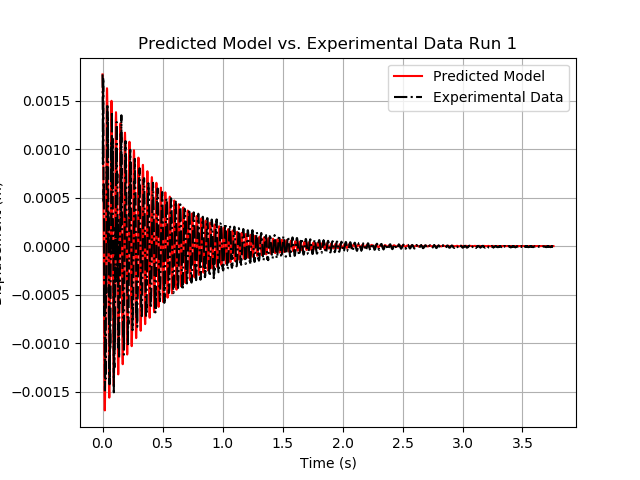
\includegraphics[width=120mm]{PEtd1.png}
\caption[your caption ref]{Predictive Model vs. Experimental Data Run 1}
\end{figure}
\begin{figure}[h!tb]
\centering
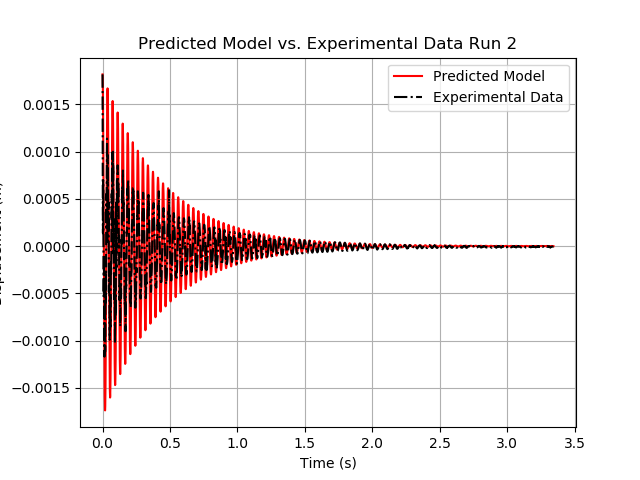
\includegraphics[width=120mm]{PEtd2.png}
\caption[your caption ref]{Predictive Model vs. Experimental Data Run 2}
\end{figure}
\newpage
\begin{figure}[h!tb]
\centering
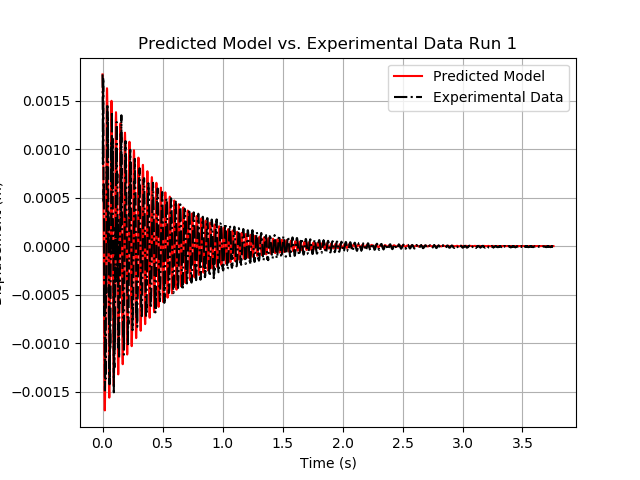
\includegraphics[width=120mm]{PEtd1.png}
\caption[your caption ref]{Predictive Model vs. Experimental Data Run 3}
\end{figure}
\begin{figure}[h!tb]
\centering
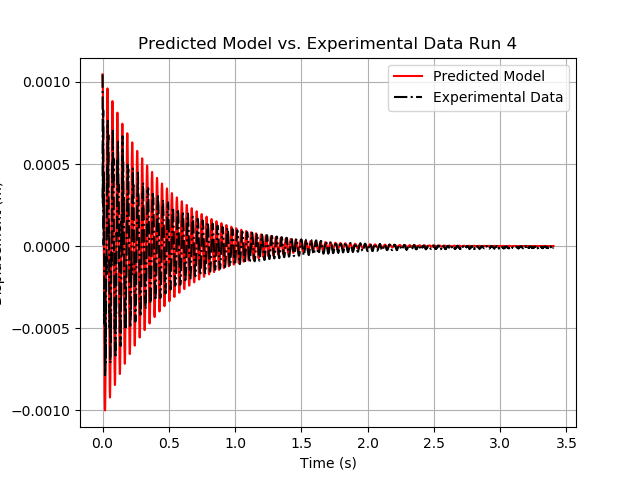
\includegraphics[width=120mm]{PEtd4.png}
\caption[your caption ref]{Predictive Model vs. Experimental Data Run 4}
\end{figure}
\newpage
\begin{figure}[h!tb]
\centering
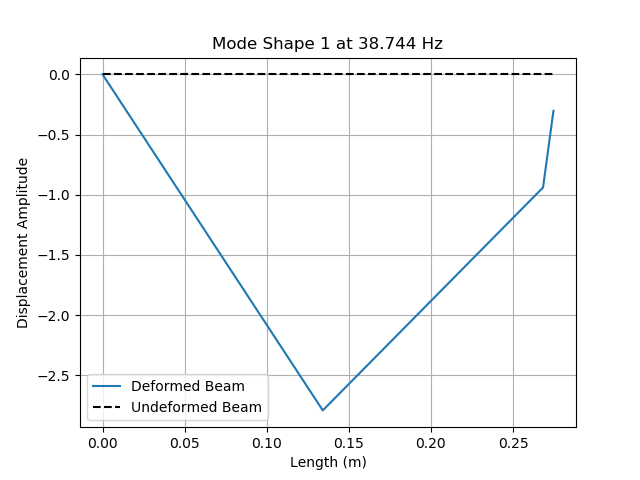
\includegraphics[width=120mm]{Mode_shape_1.png}
\caption[your caption ref]{FEA Mode Shape 1}
\end{figure}
\begin{figure}[h!tb]
\centering
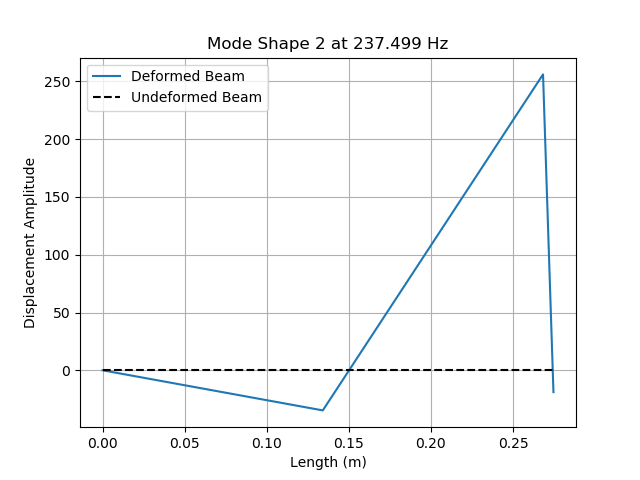
\includegraphics[width=120mm]{Mode_shape_2.png}
\caption[your caption ref]{FEA Mode Shape 2}
\end{figure}
\newpage
\begin{figure}[h!tb]
\centering
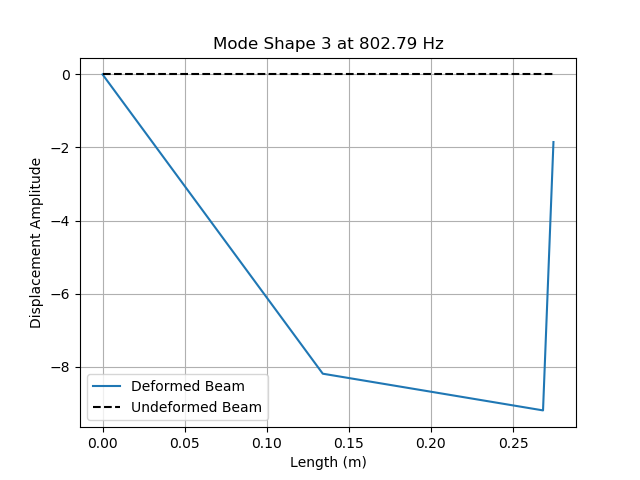
\includegraphics[width=120mm]{Mode_shape_3.png}
\caption[your caption ref]{FEA Mode Shape 3}
\end{figure}
\begin{figure}[h!tb]
\centering
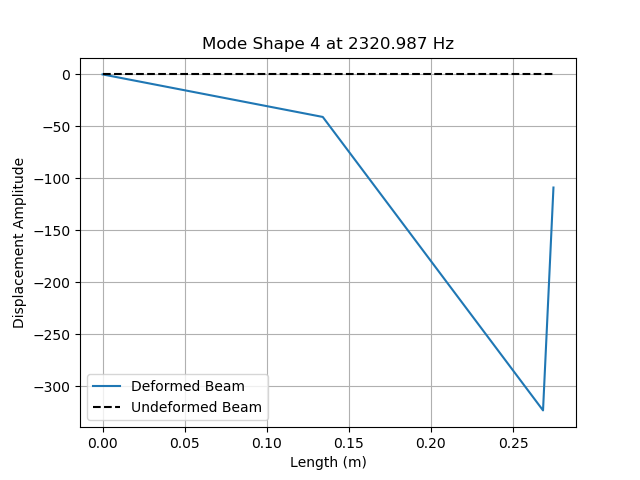
\includegraphics[width=120mm]{Mode_shape_4.png}
\caption[your caption ref]{FEA Mode Shape 4}
\end{figure}
\begin{figure}[h!tb]
\centering
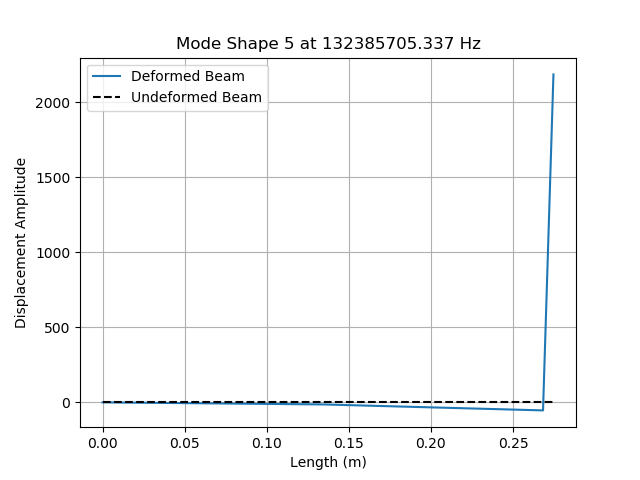
\includegraphics[width=120mm]{Mode_shape_5.png}
\caption[your caption ref]{FEA Mode Shape 5}
\end{figure}
\begin{figure}[h!tb]
\centering
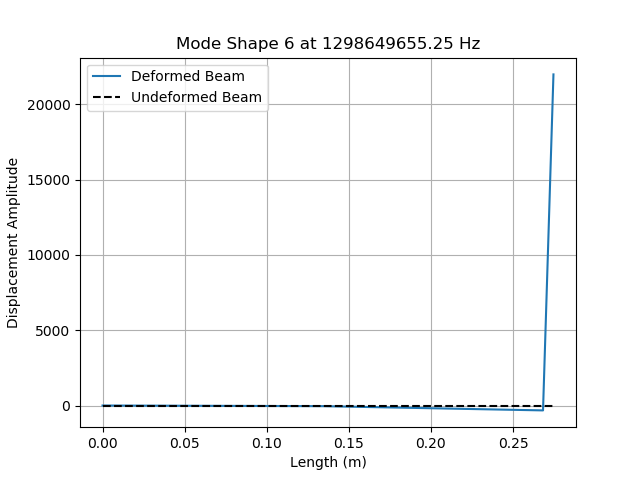
\includegraphics[width=120mm]{Mode_shape_6.png}
\caption[your caption ref]{FEA Mode Shape 6}
\end{figure}
\begin{figure}[h!tb]
\centering

\includegraphics[width=120mm]{C:/Anaconda3/My_Scripts/Controls_Lab/tv1.png}
\caption[your caption ref]{Time vs Amplitude Run 1}
\end{figure}
\begin{figure}[h!tb]
\centering

\includegraphics[width=120mm]{C:/Anaconda3/My_Scripts/Controls_Lab/tg1.png}
\caption[your caption ref]{Time vs G's Run 1}
\end{figure}
\begin{figure}[h!tb]
\centering

\includegraphics[width=120mm]{C:/Anaconda3/My_Scripts/Controls_Lab/tv2.png}
\caption[your caption ref]{Time vs Amplitude Run 2}
\end{figure}
\begin{figure}[h!tb]
\centering

\includegraphics[width=120mm]{C:/Anaconda3/My_Scripts/Controls_Lab/tg2.png}
\caption[your caption ref]{Time vs G's Run 2}
\end{figure}
\begin{figure}[h!tb]
\centering

\includegraphics[width=120mm]{C:/Anaconda3/My_Scripts/Controls_Lab/tv3.png}
\caption[your caption ref]{Time vs Amplitude Run 3}
\end{figure}
\begin{figure}[h!tb]
\centering

\includegraphics[width=120mm]{C:/Anaconda3/My_Scripts/Controls_Lab/tg3.png}
\caption[your caption ref]{Time vs G's Run 3}
\end{figure}
\begin{figure}[h!tb]
\centering

\includegraphics[width=120mm]{C:/Anaconda3/My_Scripts/Controls_Lab/tv4.png}
\caption[your caption ref]{Time vs Amplitude Run 4}
\end{figure}
\begin{figure}[h!tb]
\centering

\includegraphics[width=120mm]{C:/Anaconda3/My_Scripts/Controls_Lab/tg4.png}
\caption[your caption ref]{Time vs G's Run 4}
\end{figure}
\begin{figure}[h!tb]
\centering

\includegraphics[width=120mm]{C:/Anaconda3/My_Scripts/Controls_Lab/fft1.png}
\caption[your caption ref]{Time vs Amplitude FFT Run 1}
\end{figure}
\begin{figure}[h!tb]
\centering

\includegraphics[width=120mm]{C:/Anaconda3/My_Scripts/Controls_Lab/fft2.png}
\caption[your caption ref]{Time vs Amplitude FFT Run 2}
\end{figure}
\begin{figure}[h!tb]
\centering

\includegraphics[width=120mm]{C:/Anaconda3/My_Scripts/Controls_Lab/fft3.png}
\caption[your caption ref]{Time vs Amplitude FFT Run 3}
\end{figure}
\begin{figure}[h!tb]
\centering

\includegraphics[width=120mm]{C:/Anaconda3/My_Scripts/Controls_Lab/fft4.png}
\caption[your caption ref]{Time vs Amplitude FFT Run 4}
\end{figure}
\newpage
\section{: Python Code}
\lstinputlisting[language=Python]{C:/Anaconda3/My_Scripts/Controls_Lab/Lab_10_Analysis.py}
\newpage
\section{: Lab Outline}
(Attached On Next Page)

\includepdf[pages=-]{C:/Anaconda3/My_Scripts/Controls_Lab/Lab_10_Outline.pdf}
\end{document}